\documentclass[a4paper]{article}
\usepackage[utf8]{inputenc}
\usepackage[T1]{fontenc}
\usepackage[pdftex]{graphicx}
\usepackage{fancyhdr}
\usepackage{lscape}
\usepackage{color}
\usepackage{qtree}
\usepackage[english]{babel}
\usepackage{graphicx}
\usepackage[colorinlistoftodos]{todonotes}
\usepackage{listings}
\usepackage{color}
\usepackage{float}
\usepackage{changepage}
\usepackage[margin=1in]{geometry}
\definecolor{codegreen}{rgb}{0,0.6,0}
\definecolor{codegray}{rgb}{0.5,0.5,0.5}
\definecolor{codepurple}{rgb}{0.58,0,0.82}
\definecolor{backcolour}{rgb}{0.95,0.95,0.92}
\usepackage[final]{pdfpages} 
\usepackage[parfill]{parskip}

 
 \lstdefinestyle{mystyle}{
 	backgroundcolor=\color{backcolour},   
 	commentstyle=\color{codegreen},
 	keywordstyle=\color{magenta},
 	numberstyle=\tiny\color{codegray},
 	stringstyle=\color{codepurple},
 	basicstyle=\footnotesize,
 	breakatwhitespace=false,         
 	breaklines=true,                 
 	captionpos=b,                    
 	keepspaces=true,                 
 	numbers=left,                    
 	numbersep=5pt,                  
 	showspaces=false,                
 	showstringspaces=false,
 	showtabs=false,                  
 	tabsize=2
 }
 
\lstset{
	style=mystyle,
	inputencoding=utf8,
	extendedchars=true,
	literate={á}{{\'a}}1 {ã}{{\~a}}1 {é}{{\'e}}1,
	escapechar=\&
}
\title{Algorithmique et structures de données : Mission 5}
\date{12 décembre 2014}
\author{Groupe 1.2: Ivan Ahad - Jérôme Bertaux - Rodolphe Cambier \\ 
	Baptiste Degryse - Wojciech Grynczel - Charles Jaquet}

\begin{document}
\maketitle


Rapport écrit par Rodolphe Cambier, Ivan Ahad, Jérôme Bertaux
\section*{Introduction}
Le but de la mission est de créer un algorithme capable de faire une liste de tous les coûts minimums entre chaque noeuds, le tout sur base d'une liste de paires de noeuds et du coût de leur arête. 
\section*{Questions}

\subsection*{Question 1}
Les solutions proposées peuvent ne pas être uniques car il est possible qu'il existe plsuieurs chemins ayant un coût minimal entre deux noeuds. Les solutions sont bien optimales car l'algorithme permet de récupérer les poids minimaux des arêtes reliant les paires de noeuds. 
\subsection*{Question 2}
Notre algorithme a une complexité supérieure à la complexité théorique en O(n*log n) de l'algorithme de Kruskal où n représente le nombre d'arrêtes, car la méthode buildGraph() de notre programme fait appel à deux boucles imbriquées, qui est appelée par la méthode "KruskaAlgorithm" 
\subsection*{Question 3}

Un etechnique serait de modifier l'algorithme de Kurskal, et de faire en sorte que lorsque l'on cherche la plus petite des \textit{edges} parmis toutes celles restantes, on prenne en compte le poids des transits. Pour faire cela, il faut calculer la taille des \textit{Clusters} correspondants à chacunes des deux \textit{vertices} aux extrémités de chaque \textit{edge}, et les mutliplier, ce qui nous donnera le nombres de transits passant par cette \textit{edge}.

En prenant cela en compte, on peut continuer l'algorithme et trouver le graphe optimal,tenant en compte des transits.



\section*{Diagramme UML}
=======
Une technique serait de modifier l'algorithme de Kurskal, et de faire en sorte que lorsque l'on cherche la plus petite des \textit{edges} parmis toutes celles restantes, on prenne en compte le poids des transits. Pour faire cela, il faut calculer la taille des \textit{Clusters} correspondants à chacunes des deux \textit{vertices} aux extrémités de chaque \textit{edge}, et les mutliplier, ce qui nous donnera le nombres de transits passant par cette \textit{edge}.

En prenant cela en compte, on peut continuer l'algorithme et trouver le graphe optimal, tenant en compte des transits.


\section*{Diagramme UML}
\begin{figure}[b]
   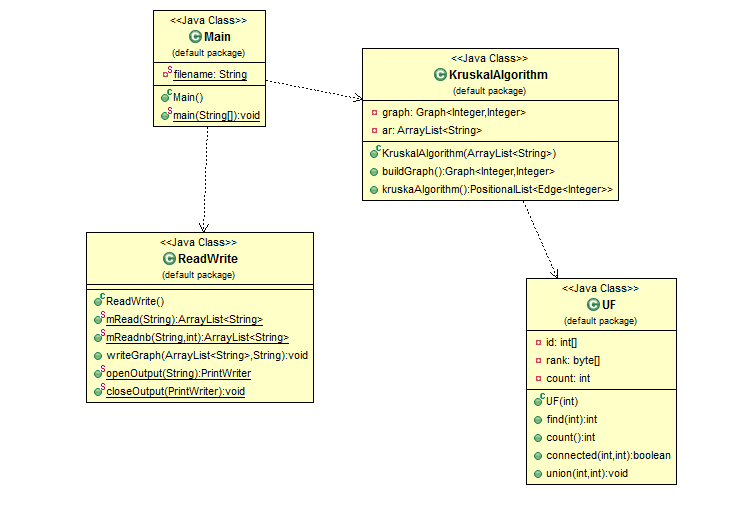
\includegraphics[scale=0.4]{UML.png}
\end{figure}

\end{document}
